\subsection{Task 2.1 -- Activity diagram}
% SVG: java -DPLANTUML_LIMIT_SIZE=16384 -jar plantuml.jar -charset UTF-8 -tsvg docs/diagrams/activity-checkout.puml
% PNG: java -DPLANTUML_LIMIT_SIZE=16384 -jar plantuml.jar -charset UTF-8 -Sdpi=200 -tpng docs/diagrams/activity-checkout.puml

\textbf{Activity-01} mô tả luồng đặt và thanh toán đơn theo SRS Task~1.2
và use-case \textbf{UC-CK} của Task~1.3.
Hình~\ref{fig:activity-checkout} chứa luồng chính và các nhánh bắt buộc
trong cùng một sơ đồ, với ba làn trách nhiệm:
\textbf{Khách hàng}, \textbf{Hệ thống (frontend/backend)}
và \textbf{Nhân viên (ADMIN)}.

\subsubsection{Luồng chính và các nhánh}

Khách xem menu, chọn size/topping, thêm món vào giỏ rồi đặt hàng.
Nếu chưa đăng nhập, hệ thống chuyển sang đăng nhập; sau khi xác thực,
khách quay lại giỏ còn nguyên và bấm đặt hàng.
Backend kiểm tra dữ liệu, tính lại giá và giữ nguyên liệu theo công thức
trong cùng transaction với optimistic locking.
Thiếu nguyên liệu thì báo lỗi, rollback và giữ giỏ; không tạo đơn.
Đơn hợp lệ được tạo ở trạng thái \texttt{PENDING}, giữ nguyên liệu
và lượt voucher trong thời hạn thanh toán 15 phút.

Hệ thống tạo phiên thanh toán \texttt{PENDING}; khách quét QR,
mở ngân hàng giả lập và bấm \emph{Chuyển tiền}.
Khi nhận tiền, hệ thống ghi sao kê \texttt{IN}, chuyển phiên sang
\texttt{TRANSFER\_RECEIVED}; đơn vẫn \texttt{PENDING}.
Nhân viên nhận thông báo qua polling mỗi 4 giây, đối chiếu sao kê
và quyết định:
\begin{itemize}
  \item \textbf{Xác nhận}: phiên \texttt{SUCCESS}, đơn \texttt{PAID};
    chốt voucher, cộng điểm. Giao diện nhận kết quả qua polling,
    xóa giỏ và hiển thị màn hình xác nhận đơn.
  \item \textbf{Từ chối}: phiên \texttt{FAILED},
    đơn \texttt{PAYMENT\_FAILED}; tự hoàn đúng khoản đã nhận bằng
    giao dịch \texttt{REFUND}; giữ nguyên liệu và giỏ.
    Nếu khách thử lại, vòng lặp trở về bước kiểm tra hạn trên
    \emph{cùng đơn}, chuyển \texttt{PAYMENT\_FAILED}
    $\rightarrow$ \texttt{PENDING} và tạo phiên với
    \texttt{Idempotency-Key} mới. Hạn vẫn tính từ lúc tạo đơn;
    không giữ nguyên liệu lần hai, không chuyển thẳng
    \texttt{PAYMENT\_FAILED} $\rightarrow$ \texttt{PAID}.
  \item \textbf{Quá hạn khi chưa nhận tiền}: tác vụ nền tự chuyển đơn
    sang \texttt{CANCELLED}, hoàn nguyên liệu và lượt voucher
    đúng một lần, giữ giỏ. Nhánh hết hạn được xử lý cả khi khách
    không thao tác hoặc quay lại thử thanh toán sau hạn.
    Đơn có phiên \texttt{TRANSFER\_RECEIVED} không tự hủy
    trong lúc chờ nhân viên.
\end{itemize}

Sơ đồ tập trung vào phương thức Ví theo luồng chính của issue~\#7.
Phương thức Thẻ tại quầy và các ngoại lệ khác được giữ theo UC-CK.
Gửi lại cùng yêu cầu do lỗi mạng dùng cùng \texttt{Idempotency-Key}
để trả lại đơn/phiên cũ; chỉ lần thử thanh toán mới sau khi bị từ chối
mới dùng key mới. Các bước xác nhận và hoàn tiền dùng transaction,
khóa dòng và kiểm tra chuyển trạng thái để tránh xử lý hai lần.

\begin{figure}[p]
  \centering
  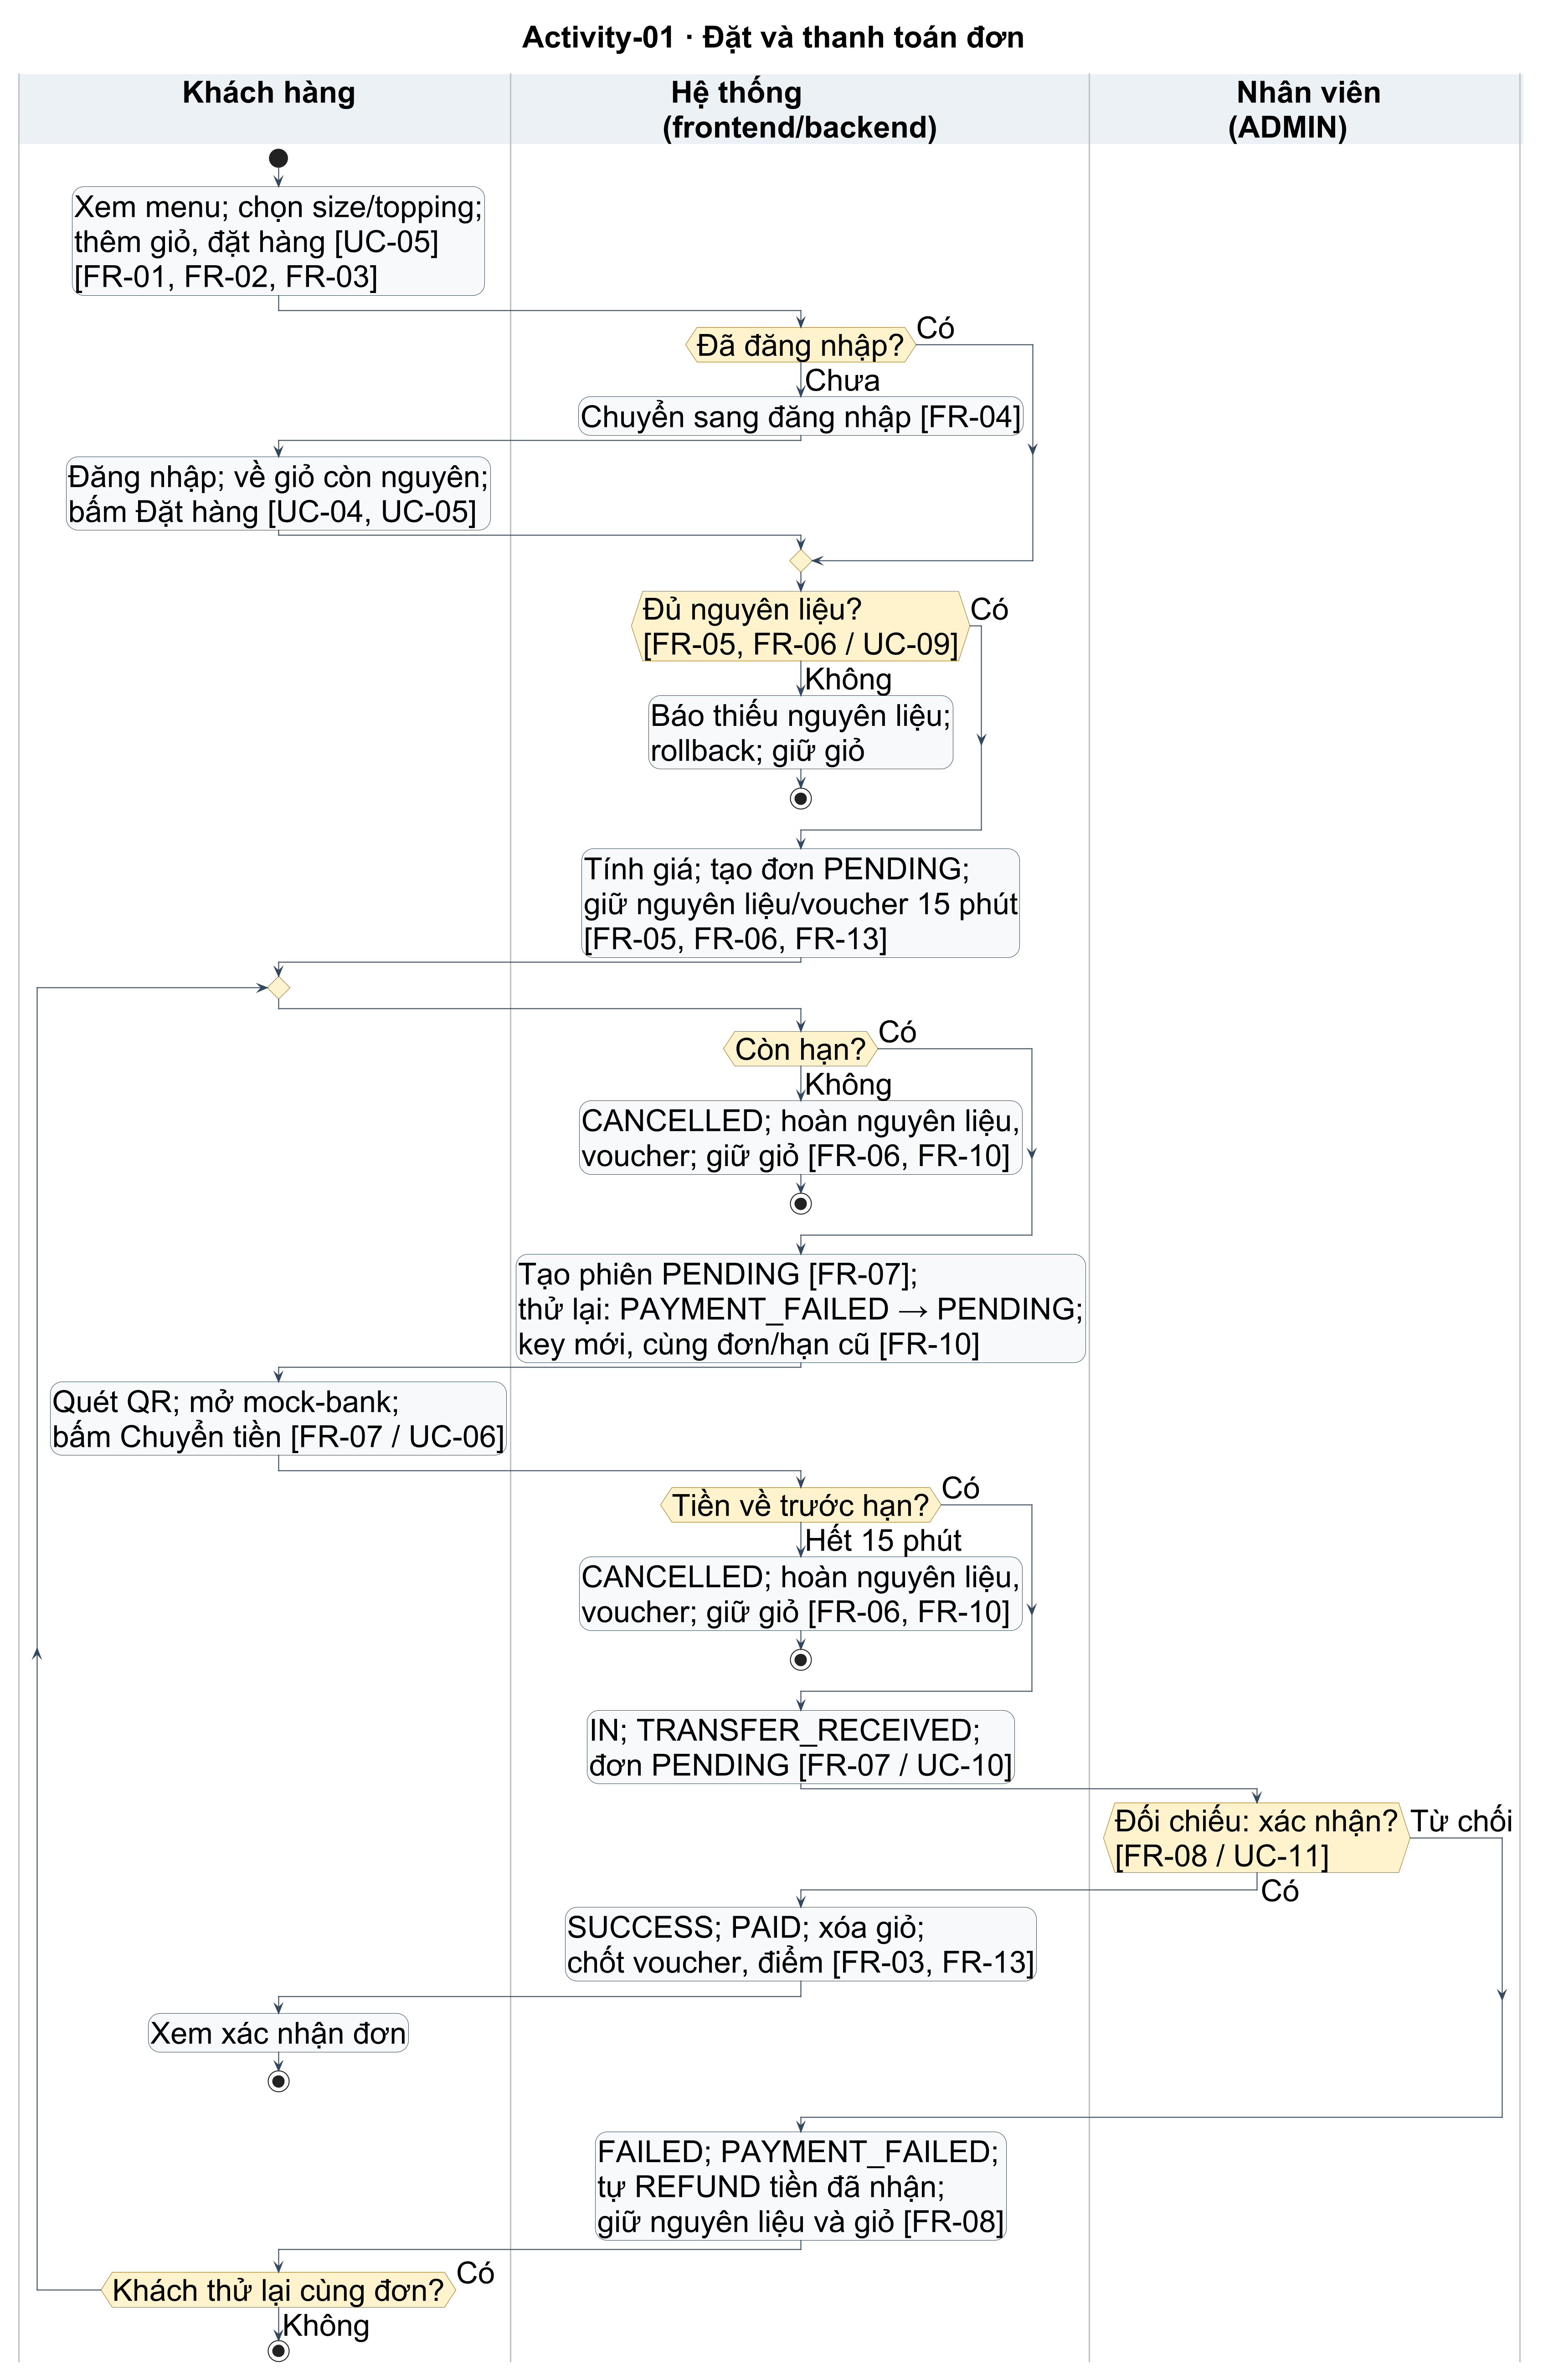
\includegraphics[width=\textwidth,height=0.93\textheight,keepaspectratio]{docs/diagrams/activity-checkout.png}
  \caption{Activity-01: Luồng đặt và thanh toán đơn, gồm đăng nhập, thiếu nguyên liệu, từ chối và thử lại, tự hủy quá hạn.}
  \label{fig:activity-checkout}
\end{figure}

\subsubsection{Truy vết yêu cầu}

Activity-01 liên kết FR-01--FR-08, FR-10, FR-13 với
UC-01--UC-06, UC-09--UC-11.
Các nguyên tắc giữ kho, chống trùng, phân quyền và phản hồi giao diện
liên quan NFR-01--NFR-03 được thuyết minh ở trên.
Cột \emph{Thiết kế / Sơ đồ} trong ma trận truy vết
chứa liên kết đến Activity-01.
